\section{Transformation of Wasm-DSL into AL}\label{sec:translate}

In this section, we describe the transformation process of Wasm-DSL into AL.
Wasm-DSL can express whole standard of the WebAssembly, including not only
execution semantics but also syntax and validation rules.
Since the main goal of this paper is to generate prose from execution semantics but not syntax or validation,
we will focus on how only execution semantics of Wasm is expressed using Wasm-DSL.

\subsection{Notations}

Two kinds of \textit{definitions} are needed to express the execution semantics of Wasm:
reduction rules and auxiliary helper functions.
Here, we formally define the notations for the reduction rules and the auxiliary helper functions.

First, assume that the set of DSL expressions $E$ and boolean expressions $B \subset E$ are given.
DSL expressions are basic building building blocks of DSL, including number, identifiers,
function calls, pairs, operations between them, etc. \inred{How much detail is needed for DSL expressions?}

A reduction rule $\ruleW \in \rulesW = \configsW \times \configsW \times \premsW^\ast$ is a triplet of a
configuration \textit{lhs}, a configuration \textit{rhs}, and a finite sequences of premises \textit{prem}*.
The high-level interpretation of a reduction rule $r = (lhs, rhs, prem*)$ should be straightforward:
when the current configuration of the program matches \textit{lhs} and all \textit{prem}s are
evaluated to be true, then alter the program configuration into \textit{rhs}.

A configuration $\configW \in \configsW = E_\bot \times E$ is a tuple of an optional expression for state \textit{z},
and an expression for a finite sequence of Wasm instructions, \textit{winstrs}.
\textit{z} is a syntactic representation of the internal state of the program. Specifically for WebAssembly,
a state is a pair of the current \textit{store} and the current \textit{frame}. A naive, high-level
interpretation of \textit{winstrs} is that it represents the current \textit{stack}, which grows right.
Thus, the last element of winstrs represent the top of the stack.

A premise $p \in \premsW = B \uplus \{otherwise\}$ is either a boolean expression, or a
single `otherwise` whose high-level interpretation is "negation of all previous premises".

\textbf{Example.} Recall the semantics of `ref.is\_null` in figure~\ref{fig:dsl1}.
The first rule will be parsed into the following reduction rule:
\[r_1=(\bot, [val, \text{REF.IS\_NULL}]), (\bot, [\text{CONST I32 1}]), [val = (\text{REF.NULL rt})]\]
The second rule will be parsed into the following:
\[r_2=(\bot, [val, \text{REF.IS\_NULL}]), (\bot, [\text{CONST I32 0}]), [otherwise]\]
Note that both of lhs and rhs for both rules are omitting the state expression,
and thus we notate it by using $\bot$.

A helper function $\helperW \in \helpersW = Id \times E^\ast \times E \times \premsW^\ast$ is a quadruple of
the name, parameters \textit{params}, a return expressions \textit{ret}, and a finite sequences of premises \textit{prem}*.

\textbf{Example.} `default` is an auxiliary helper function that takes a Wasm type as an input, and yields
the default Wasm value (usually zero) of that type as an output. The following is the
DSL that represents the two cases for this function:

\inred{TODO: Pretty print this}

-------------------------

\texttt{
def \$default\_(t) = (CONST I32 0)
}

\texttt{
-- if t = I32
}

\texttt{
def \$default\_(t) = (CONST I64 0)
}

\texttt{
-- if t = I64
}

-------------------------

When the type `I32` is given, `CONST I32 0` should be returned,
and when the type `I64` is given, `CONST I64` should be returned.
These definitions will be parsed into the following:
\[h_1=\text{"default\_"}, [t], \text{(CONST I32 0)}, [t = \text{I32}]\]
\[h_2=\text{"default\_"}, [t], \text{(CONST I64 0)}, [t = \text{I64}]\]


\subsection{Transformation}

\begin{figure}
  \centering
  \begin{subfigure}[b]{0.9\textwidth}
    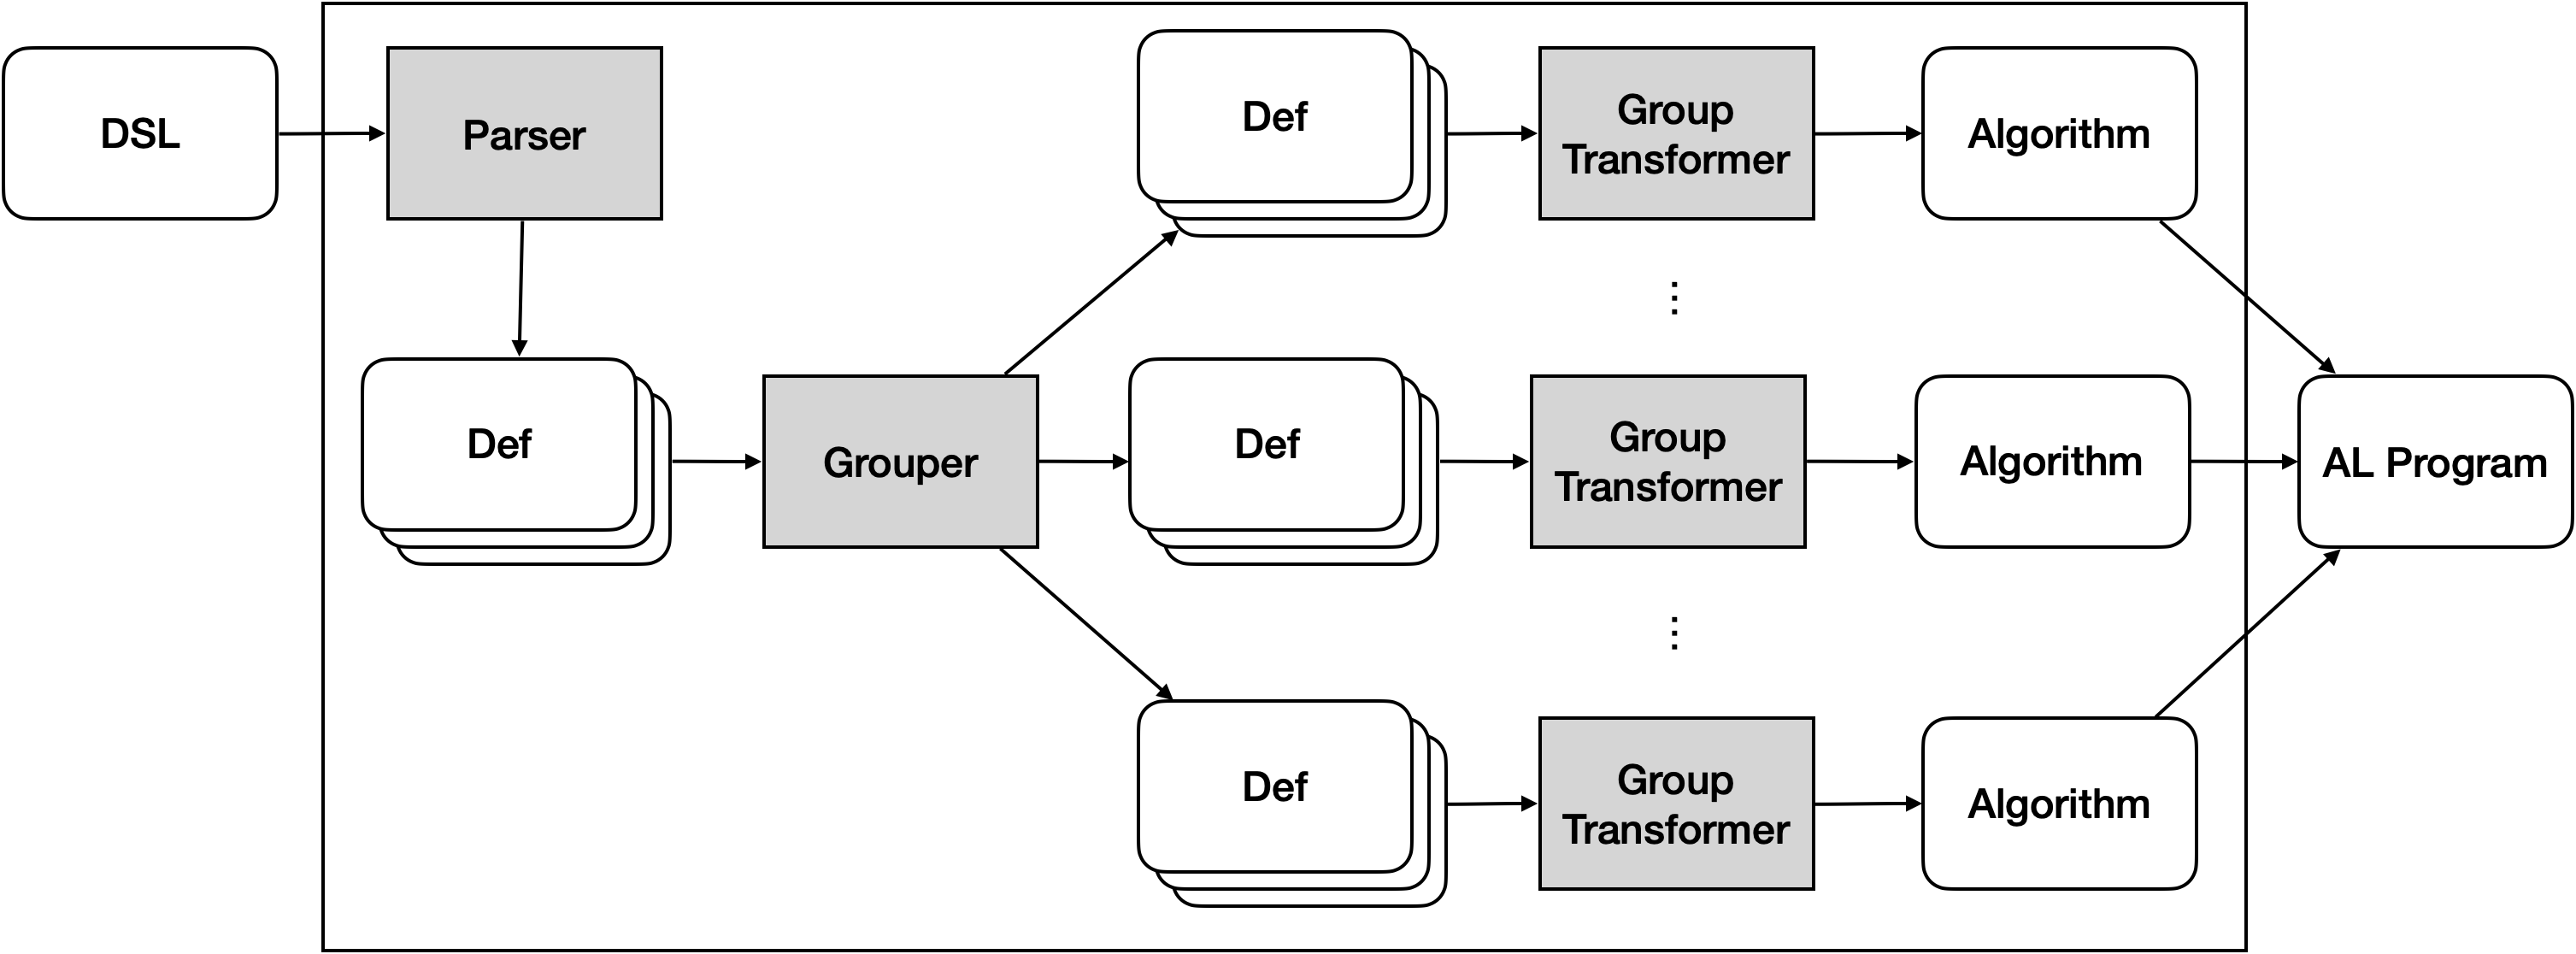
\includegraphics[width=\textwidth]{img/trans1}
    \caption{Overview}
    \label{fig:overview}
  \end{subfigure}
  \hfill
  \begin{subfigure}[b]{0.9\textwidth}
    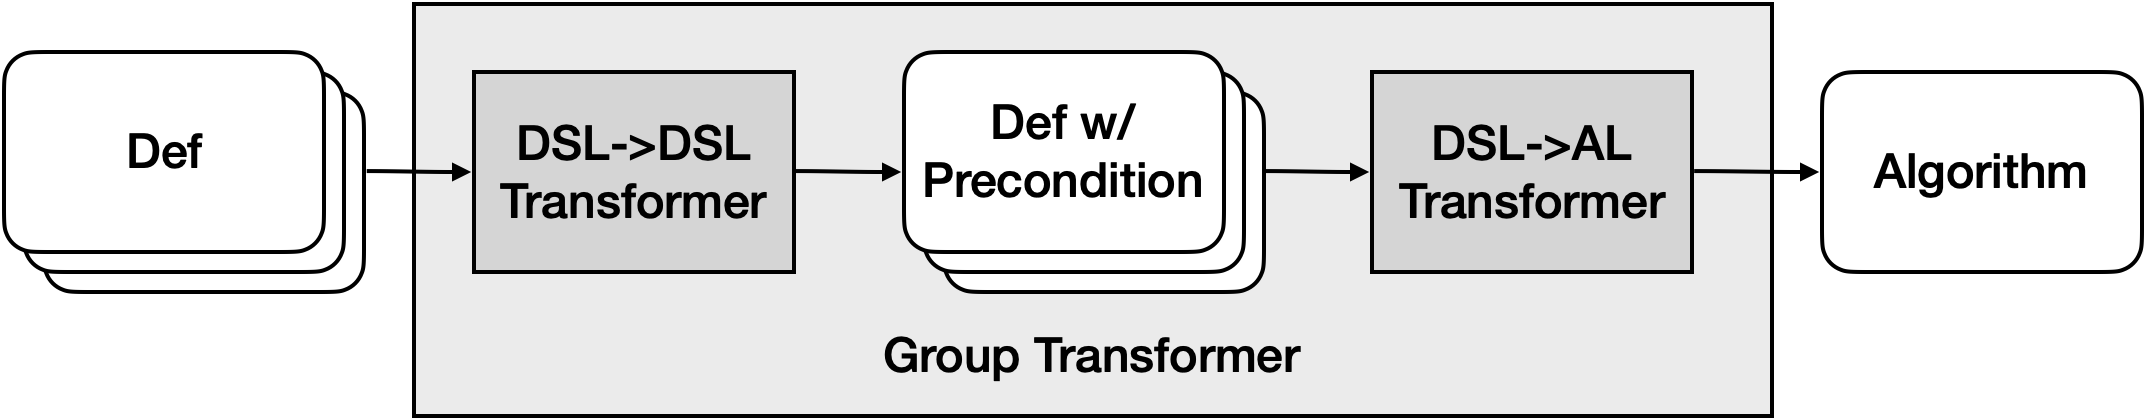
\includegraphics[width=\textwidth]{img/trans2}
    \caption{Group transformer}
    \label{fig:grouptrans}
  \end{subfigure}
  \caption{DSL->AL transformation}
  \label{fig:trans}
\end{figure}

In this section, we describe the transformation of \dsl~into \al.
Figure~\ref{fig:overview} shows the whole system of transforming DSL into an \al~program.
The input of the system is the \dsl~document,
and the output of the system is a single \al~program $\mathsf{p}$.
The input undergoes the following process of transformation.
First, the input DSL is parsed into a set of definitions: either a reduction rule or a
helper function. Then, the definitions are grouped.
A group represents the set of definitions that should be bundled and transformed
into a single algorithm together.
Reduction rules are grouped based on
their target Wasm instruction, and helper functions are grouped based on their names.
As a result, multiple groups are formed. Each group is transformed into a single algorithm,
$\mathsf{A}$. The transformed algorithms are collected into a single AL program, which is the
final output of this transformation system. This AL program then can be stringified into a
prose notation specification document, or can be coupled with the AL interpreter to form a Wasm interpreter.

Figure~\ref{fig:grouptrans} shows the detail of group transformer, a component of the Figure~\ref{fig:overview}.
The input is either a group of reduction rules \textit{r}, or a group of helper functions \textit{h}.
The output is a single algorithm.
Due to the fundamental difference between mathematical rules and algorithm,
directly transforming into an algorithm is a non-trivial task.
Therefore, the process is divided into two steps: first pre-process DSL so that
it becomes more suitable for transformation, and then transform it into an algorithm.
As a first step, a group of definitions are first pre-processed into a
different group of definitions in semantics-preserving manner,
so that the new pre-processed group of definitions satisfies certain \textit{preconditions}.
The preconditions will be helpful when generating AL algorithms.
If the input group already satisfies the precondition, then this transformation will keep the input intact.
Secondly, Then new group of definition is transformed into AL.
How the AL is generated slightly differ based on whether the group is a reduction rule group or a helper function
group, but they are both based on the following fundamental approach.
% Should I explain AL -> AL?

~

\subsubsection{\textbf{DSL->DSL pre-processing}}~

The first step of the transformation is to pre-process DSL into a one that meets certain preconditions.
There are two major pre-processing: 1. Unification and
2. Animation.

\textbf{1. Unification}

Unification is a step that makes all LHS (for reduction rule) or parameters
(for helper functions) identical within the group.
This precondition already holds for most cases, with a few exceptions.
The most notable example is the `br` instruction.
Here are two simplified reduction rules for the `br` instruction
\[
r_1 = (..., [... \text{(BR 0)} ...]),  (..., ...), []
\]
\[
r_2 = (..., [... \text{(BR l+1)} ...]),  (..., ...), []
\]
The intention here is that `BR l` instruction should be applied with different rule,
depending on whether $l$ is 0 or not.
Note that the both rules do not have any premise. The condition check is implicitly assumed to be
done when matching the current configuration with LHS.

The following is the result of unification:
\[
r_1' = (..., [... \text{(BR t)} ...]),  (..., ...), [t = 0]
\]
\[
r_2' = (..., [... \text{(BR t)} ...]),  (..., ...), [t = l + 1]
\]
The temporary variable $t$ is introduced for both rules, replacing 0 of the first rule and
$l+1$ of the second rule. In order to denote what the temporary variable originally was
in each rules, new premise is added, denoting $t$ equals 0 in the first rule, and $l+1$ in the second rule.

----------------

Algorithm 7. Unification

Input: A list of DSL expressions e*

Output: A unified DSL expression e, a list of premise sequnces p**

1. template <- fold\_left(unify\_two)(e*)

2. For i < |e*|:

  a) p**[i] <- extract\_prems(e*[i], template)

3. Return (template, p**)

----------------

----------------

Helper: unify\_two

Input: Two DSL expressions e1, e2

Output: Unified DSL expression e

1. If e1 is idenical with e2:

  a) Return e1

1. If e1 and e2 have different grammar production:

  a) Return fresh\_var()

2. e1'* <- sub\_exprs(e1)

3. e2'* <- sub\_exprs(e2)

4. e'* <- unify\_two*(e1*, e2*)

5. Return e1 after replacing subexpressions e1'* with e'*, respectively

----------------

----------------

Helper: extract\_prems

Input: Two DSL expressions e, e\_t

Output: A list of premises p*

1. If e1 is idenical with e2:

  a) Return []

1. If e1 and e2 have different grammar production:

  a) Assert: e\_t is a fresh variable generated by fresh\_var

  a) Return [`e\_t = e`]

2. e1'* <- sub\_exprs(e1)

3. e2'* <- sub\_exprs(e2)

4. Return flatten(extract\_prems*(e1*, e2*))

----------------

Algorithm 7 shows the detaield description of the unification process.
The input is a list of a expressions to be unified: the lhs for reduction rule group, and the parameter
sequence for the helper function group.
The unification is performed in two phases: Creating a the unified expression \textit{template} which may
contain new fresh variables, and aplying the template to extract premises to be added for each definition.
As a resuslt, the output of the algorithm is a tuple of tthe template, and the list of extracted premise sequence.
To begin with, the template is calculated by fold-lefting the expressions
with the unify\_two helper function (i.e. template <- e1 + e2 + ... + en,
where + symbol denotates unify\_two helper function) on line 1.
In a high-level, the unify\_two helper function is a function that given two expressions,
spots the difference between them and replace the differences with fresh vaiables. It works by
traaversing two ASTs of expressions simultaneously, until they are totally identical or
has different grammar production.
After the template is calculated, the new premises that handles fresh variables are extracted
in the loop on line 2. This is done by callig extract\_prems helper function. In a high-level,
this function compares the template and the expression, and extract the premise that identifies the
generated fresh variable in the template, and the corresponding sub-expression for the given expression.
This helper function also use the strategy of traversing two ASTs simultaneously. Once the premises are
extracted, the tuple of the template and the premise sequnce list is returned as the final result on line 3.
These information will be used to generate the pre-processed definition group, by
replacing the expresions (lhs or parameters) with the template, and appending additional
premises to the original premises.


\textbf{2. Animation}

There are two problems that makes it challenging to transform premises into AL.
First, if a given premise is an equality expression, then it may work as either a simple condition or
a binding of a new variable, and this should be inferred. More formally, it is required to
correctly find out where each free variable is getting bound. Second, the order
of premises can be permutated in an arbitrary order. This is problematic for
generating algorithm, since the exact order of steps are crucial in the algorithm.

Animation is a step that addresses these two challenges. Its goal is to infer
the bound variables and the order of each premise.
After animation, each premise is tagged with what variables it is binding
such that every variables are bound exactly once, and premises are ordered in a way that
all of unbound variables in each premise is already bound by the previous premises.

Let's look at the BR example again:
\[
r_1' = (..., [... \text{(BR t)} ...]),  (..., ...), [t = 0]
\]
\[
r_2' = (..., [... \text{(BR t)} ...]),  (..., ...), [t = l + 1]
\]
In the first rule, the premise t = 0 is the equality check.
In the second rule, on the other hand, the premise $t = l+1$ is actually a binding of $l$ with a new value.
Therefore, the animation process will preserve the first rule as it is, but will change the
second rule into the following:
\[
r_2'' = (..., [... \text{(BR t)} ...]),  (..., ...), [l + 1 \leftarrow t]
\]
which clearly indicates that the new variable $l$ is a new introduced variable.
Now, in order to illustrate the effect of premise ordering, let's think of 
hypothetical additional premises that contains the variable $l$, i.e.,
\[
r_2'' = (..., [... \text{(BR t)} ...]),  (..., ...), [l + 1 \leftarrow t]
\]
the animation process will make sure that the premise $(l + 1 \leftarrow t)$ will be
placed before them.

We have discovered that solving the animation problem is in fact NP-hard.
This is especially because a single premise can bind more than two variables at once, as in
$(x,y) \leftarrow p$.
We prove it by reduction from a known NP-hard problem, the \textit{exact cover} problem.

\textbf{Definition.} Partition: Given a set $X$, a collection\footnote{Throughout the paper, we will
use a convention of notation that a collection means a set of sets.}
of subsets of $X$, $P \subset 2^X$, is a partition of $X$ iff
1. The union of all sets in $P$ is $X$,
2. All sets in $P$ are pairwise disjoint.

For example, $P$ = \{\{a,b\}, \{c,d\}, \{e\}\} is a partition of the set $X$ = \{a, b, c, d, e\},
since 1. the union of all sets is X, and 2. any pair of subsets are disjoint.

\textbf{Definition.} Exact cover problem: Given a set $X$ and a collection $S \subset 2^X$,
exact cover problem is a decision problem to determine if there exists a partition $P$ which is a
subcollection of S.

For example, consider a collection $S = \{\{a,b\}, \{b,c\}, \{c,d,e\}\}$.
One of it's subcollection, $\{\{a,b\}, \{c,d,e\}\} \subset S$ is a partition of $X$,
so the answer to the problem is YES.
On the other hand, given a collection $S' = \{\{a,b\}, \{b,c\}, \{c,d\}, \{d,e\}\}$,
no any subcollection of $S'$ is a partition of $X$\footnote{It can be easily
verified by the parity. The union of any pair-wise disjoint subcollection of $S'$ would have an even number
of elements, but the whole set $X$ has 5 elements.}, so the answer to the problem is
NO.

Exact cover problem is a well-known NP-complete problem and is one of Karp's 21 NP-complete problems[?].
Therefore, we can prove that animation problem is NP-hard, if we reduce Exact cover problem
into animation problem in polynomial time.

\textbf{Theorem}: Animation problem is NP-hard.

\textbf{Proof}: Let's assume we are given a exact-cover problem with a set $X$ and a
collection of its subset, $S \subset 2^X$. Let n be size of $S$.
Let $S_i = \{x_{i1}, x_{i2}, ..., x_{ij}\}$ be the i-th subset of S.
Now, consider the reduction rule $(lhs, rhs, prems)$ where
$lhs$ is $(\top, [val_n, val_{n-1}, ..., val_1])$,
$rhs$ is $(\top, [])$, and
i-th premise of $prems$ be $val_i = (x_{i1}, x_{i2}, ..., x_{ij})$.
Note that this reduction rule can be constructed in linear time.
The claim is that when this rule is animated properly, this gives a solution to the exact-cover problem.
After animation, some premises will be explicitly annotated to be a variable bindings,
and they will be ordered in front of other premises. Note that the requirement for the
bound variables is that every variable must be bound exactly once. Therefore, if we collect
all premises denoted to be bounding, then the subsets $S_i$ corresponding to each bounding premises
would form a subcollection of S, which is a partition of the set $X$.

\textbf{Example.}
Let's consider the example of $X = \{a, b, c, d, e\}$ and $S = \{\{a,b\}, \{b,c\}, \{c,d,e\}\}$ again.
Following the proof above, the exact cover problem for X and S is reduced to the animation problem for the
following reduction rule:
\[r = (\top, [val_3, val_2, val_1]), (\top, []), [val_1 = (a,b), val_2 = (b,c), val_3 = (c, d, e)]\]
If we successfully solve the animation problem, then the result should look like the following:
\[r' = (\top, [val_3, val_2, val_1]), (\top, []), [(a,b) \leftarrow val_1, (c, d, e) \leftarrow val_3, val_2 = (b,c)]\]
From the result, we can reconstruct the partition of the set $X$ by looking at first two bindings,
$\{\{a, b\}, \{c, d, e\}\}$, giving the answer to the exact cover problem.

This theorem implies that there is no polynomial time algorithm for solving this problem, and a
simple bure-force would not be sacalable enough to be applied to larger number of premises.
One typical solution to this kind of problem is probably using a SMT solver such as Z3[???], since
this problem is fundamentally a constraint problem.
However, using such a heavy tool seems to be a bit over-engineering for this rather small input.
Instead, we decided to use a simple yet effective approach.
We reduce the problem into a exact cover problem\footnote{Note that the direction is opposite with
the proof}, and then adopt the well-known effective algorithm to solve exact cover problem,
the Knuth algorithm[?]. The high-level idea is to encode the premises into a
collection of sets, where the solution for the exact cover problem on the encoded set
would corresponds to the correct animation result.

----------------

Algorithm 0. Premise inferecne

Input: A list of premises prems, a set of bound variables vars

Output: A list of animated premises prems'

1. S <- \{\}

2. For i in |prems|:

-- a. If prems[i] == `(lhs = rhs)`:

---- 1) S\_i = \{\{i\}, \{i\} $\cup$ free(lhs), \{i\} $\cup$ free(rhs)\}

-- b. Else:
    
---- 1) S\_i = \{\{i\}\}

-- c. S <- S $\cup$ S\_i

3. Let partitions <- knuth(S $\cup$ \{vars\})

4. For partition in partitions:
  
-- a. prems' <- annotate(prems, partiton)

-- b. If reorder(prems') succeeds:

---- 1) Return reorder(prems')

----------------

----------------

Helper: Annotate

Input: A list of premises prem*, A partition p

Output: A list of annotated premises prem'*

1. For i in |prem*|:

-- a. If prem[i] == `(lhs = rhs)`:

---- 1) If \{i\} $\in$ p:

------ a) prem'[i] <- `(lhs = rhs)`

---- 2) Else if \{i\} $\cup$ free(lhs) $\in$ p:

------ a) prem'[i] <- `(lhs <- rhs)`

---- 3) Else if \{i\} $\cup$ free(lhs) $\in$ p:

------ a) prem'[i] <- `(rhs <- lhs)`

2. Return prem'*

----------------

----------------

Helper algorithm: Reorder

Input: A list of premises prem*, a set of bound variables vars

Output: A list of reordered premises prem'*

1. prem'* <- []

2. Repeat:

-- a. (p1*, p2*) <- extract\_bound\_conds(prem*, vars)

-- d. (p3*, p4*) <- extract\_bound\_bindings(p2*, vars)

-- c. prem'* <- prem'* ++ p1* ++ p3*

-- d. If p4* is empty:

---- 1) Return prem'*

-- e. Else if p3* is empty:

---- 1) Fail.

-- f. prem* <- p4*

-- g. vars <- vars $\cup$ free(lhs\_of(p3*))

----------------

Alogorithm 0 explains about the process.
Two inputs are given: the list of premises to be animated, and the set of vriables that are already bound.
In a reduction rule, all free variables appearing in the left-hand side are conidered to be bound,
and for a helper function, all free variables appearing in the parameters are considered to be bound.
The output of the algorithm is the animated (annoatated and reordered) list of premises.
The step from line 1 to 2 is encodes premises into a collection of subset of $X$,
where $X = \{1, ..., n = |prems|\} \cup free(prems*)$ is a set containing the number from 1 to the size of
premesis $n$, and all free variables appearing in premises.
on which the Knuth algorithm will be performed. The collection S is initilized as an empty collection on
line 1, and is populated by the encoded subsets of $X$ for each premises on loop of line 2.
In each loop, the i-th premise prem[i] is transformed into a collection of one or
more subsets, depending on its form. If the premise has the form of a equalty `lhs = rhs` as on line 2-a,
then the premise is encoded into three sets: \{i\}, \{i\} $\cup$ free(lhs), \{i\} $\cup$ free(rhs). The subset encodes
the possible interpretations about i-th premise. The first set \{i\} denotes that
the i-th variable does not bind any variables, meanig i-the premise is a condition.
The set \{i\} $\cup$ free(lhs) denotes that the i-th premise binds all the variable in left-hand
side of the equality, and similarly for \{i\} $\cup$ free(rhs). For example, if `x=y` is the first premise,
it sould be enocded in three subsets: \{1\}, \{1, x\} and \{1, y\}. If the given premise was not equality,
then the branch on line 2-b is taken and the premise is encoded into a single set, \{i\}, meaning
that i-th premise would definitely bind no variables, meaning it works is a condition checking premise.
For instace, if the second premise is `x < y`, then it will be endoded into only one set: \{2\}.
On line 3, the collection S, containing all of the encoded subsets and additional one subset consisting of
all already bound variables, is given to the knuth algorithm. The knuth algorithm will
effectively find the partitions of S. Note that the partition of a collection may not be uique, and
more than one partitons may be returned. Note that for any partiton p, due to the definition of partiton,
there should be exactly one subset that contains a number i for all 1 <= i <= n. Thanks to the
design of encoding, the subset is either a singleton set \{i\} or a set with other variables,
\{i, var1, var2, ...\}. On line 4-a, the algorithm annotate the premises based on this information by calling
the helper function Annotate. In a high-level, what the helper function does is to annotate whether
the i-th premise is a condition or
a variable binding, depending on what subset is included in the given partition. For example, if the
subset {1} is included in the partiton, then the first premise will remain as `x = y`, but if the
subset {1, y} is present, then the first premise will be transformed into the binding `y <- x`.
Afther the annotation is done, the final step is to reorder the premises, which is done by calling the helper
function reorder on line 4-b. It reorders the premises in a way that whenever a premise binds a new variable,
any other premises that use the variable to appear after it.
In a high-level, the helper function works by iteratively extracting completely bound
conditions and variables, which are safe to be placed in the front of the premise list.
If successful, the reordered premises will be returned as the final result on
line 4-b-1.  The reordering may fail, if the premises contaian a cyclic
definition.  For example, the list of premises {x=f(y), y=g(x)} would be
annotated \{x<-f(y), y<-g(x)\}, but it is impossible to correctly reorder them. 


\subsubsection{\textbf{DSL->AL transformation}}~

In this section, we explain the transformation of pre-processed DSL into an AL algorithm.
We will explain the transformation in top-down manner:
first explain the flow of top-level algorithm,
and then detail expression for each sub-algorithms.

----------------

Algorithm 1. rule\_to\_algo

Input: A group of reduction rules r* = (lhs, rhs, prems)*

Output: An algorithm $\mathsf{A}$

1. lhs <- r*[0].lhs

2. instrs <- lhs\_to\_instrs(lhs)

3. For r in r*:

--a. prems = r.prems

--b. rhs = r.rhs

--c. instrs\_prems <- prems\_to\_instrs(prems)

--d. instrs\_rhs <- rhs\_to\_instrs(rhs)

--e. instrs <- instrs ++ append\_at\_innermost(instrs\_prems, instrs\_rhs)

4. (name, params) <- extract\_name\_and\_params(lhs)

5. Return ($\mathsf{algorithm}$ name (params) {instrs})

----------------

\inred{TODO: Pretty print algorithm 1}

After the group is pre-processed, the next step is to transform the group into
an algorithm. Algorithm 1 depicts the pseudocode of the transformation of group
of reduction rules into an algorithm.  First, the lhs of this reduction rule
group is extracted on line 1, and is transformed into an AL instructions on
line 2. Due to the pre-condition, it is guaranteed that every lhs of reduction
rule are identical and any lhs from any rules of the group can be used. In the
algorithm, lhs of the first rule (r*[0]) is used. The result of this
transformed lhs will be used as an initial instruction list, and will grow
iteratively by the loop that iterates over each rule on line 3.  For each rule,
premises and rhs are extracted on line a and b respectively, and then
transformed into instructions on lines c and d respectively. These two lists of
instructions are merged to form a single list of instructions by appending the
rhs-instructions into the innermost block of prems-instructions,
and then appended to the initial instruction list on line e.  Finally, the name and
parameter of this algorithm is extracted from the lhs of the reduction rule on
line 4. At last, the name, parameters, and AL instructions will be packed and
returned as the final algorithm.

\textbf{Example.} Recall the reduction rules for `REF.IS\_NULL` again:

\[r_1=(\bot, [val, \text{REF.IS\_NULL}]), (\bot, [\text{CONST I32 1}]), [val = (\text{REF.NULL rt})]\]

\[r_2=(\bot, [val, \text{REF.IS\_NULL}]), (\bot, [\text{CONST I32 0}]), [otherwise]\]

When this group of reductions is given as an input to the Algorithm 1, the following steps are taken.
First, the common lhs $(\bot, [val, \text{REF.IS\_NULL}])$ is extracted from line 1.
Then, this lhs will be transformed into the AL instructions by line 2:
\[[\mathsf{assert} ...,~\mathsf{pop}~val]\].
Next, we look at the first reduction rule and extract its premises and rhs on line a and b:
$ [val = (\text{REF.NULL rt})], (\bot, [\text{CONST I32 1}])$.
The premise is transformed into an $\mathsf{if}$ instruction on line c:
\[[\mathsf{if}~(val = \text{REF.NULL rt})~[]]\]
and the rhs is transformed into a $\mathsf{push}$ instruction on line d:
\[[\mathsf{push}~\text{(CONST I32 1)}]\]
The $\mathsf{push}$ instruction is then appended to the then-branch of the $\mathsf{if}$ instruction on line e:
\[[\mathsf{if}~(val = \text{REF.NULL rt})~[\mathsf{push} \text{(CONST I32 1)}]]\]
and the final $\mathsf{if}$ instruction will be appended after lhs-instruction.
In similar fashion, the premises and rhs of the second rule will be translated into the following:
\[[\mathsf{if}~\text{otherwise}~[\mathsf{push} \text{(CONST I32 0)}]]\]
By concatenating all of the generated AL instructions, we get this final result:
\[[
\mathsf{assert} ...,~
\mathsf{pop}~val,~
\mathsf{if}~(val = \text{REF.NULL rt})~[\mathsf{push}~\text{(CONST I32 1)}]~[\mathsf{push}~\text{(CONST I32 0)}]
]\]
Finally, we extract the name and the parameters for the algorithm, which is obtained by looking at
the target instruction, `REF.IS\_NULL`. Here, the name of algorithm is simply same as the instruction tag,
`REF.IS\_NULL`, and since this instruction does not get any other parameter (unlike `br`), the parameter of
the algorithm is also a empty list. As a result, the triplet of name, parameters, and body instructions will form
the AL algorithm.
By stringifying this algorithm into a prose, we can get the result that resembles the prose notation in
Figure~\ref{fig:prose1} very closely.

From now on, we explain three main sub-algorithms for the algorithm 1,
which transform lhs, rhs, and premises into AL instructions.

----------------

Algorithm 2. lhs\_to\_instrs

Input: A left-hand side expression $lhs = (z, winstrs)$

Assumption: Exactly one of target\_is\_on\_top (winstrs) or target\_is\_in\_context (winstrs) holds.

Output: A list of AL instructions $instrs$

1. header <- state\_to\_instrs(z)

2. If target\_is\_on\_top (winstrs)

-- a. [v\_n v\_n-1 ... v\_1 winstr] <- winstrs

-- b. instr\_i <- $\mathsf{pop}$ v\_i (for 1 <= i <= n)

-- c. Return [instr\_1, instr\_2, ..., instr\_n]

3. Else if target\_is\_in\_context (winstrs)

-- a. [ C[v\_n v\_n-1 ... v\_1 winstr \_] ] <- winstrs

-- b. instrs\_context <- context\_to\_instrs(C)

-- c. instr\_i <- $\mathsf{pop}$ v\_i (for 1 <= i <= n)

-- d. Return append\_at\_innermost (instrs\_context, [instr\_1, instr\_2, ..., instr\_n])

----------------

\textbf{lhs\_to\_instrs} Algorithm 2 depicts the detail of lhs\_to\_instrs sub-algorithm.
The transformation is based on an assumption that holds for every lhs of current Wasm reduction rules:
\textit{winstrs} is either 1) a list of several Wasm instructions with the target instruction at the top of the stack,
or 2) a single \textbf{context} with the target instruction at somewhere inside it.

The first form has the following structure:
\[
w\_instrs = v_n v_{n-1} ... v_1 winstr
\]
For most of the existing rules for current version of Wasm semantics, including the one in the figure~\ref{fig:formal1}),
lhs has this form.

The second form has the following structure:
\[
w\_instrs' = C[v_n v_{n-1} ... v_1 winstr \_]
\]
Here, $C$ represents a \textit{context}. We define a context as a Wasm instructions that
can contain other Wasm instructions inside it. Currently, there are only two kinds of
contexts that actually appear in the left-hand side of the reduction rules of the
current version of Wasm semantics: \textit{Label} and \textit{Frame}.
The rules that have the second form are relatively rare.
In fact, there are only 2 exceptions: `br` and `return`, whose reduction rules
have the second form.

The following is the process of the algorithm.
When the input $lhs = (z, winstrs)$ is given, the algorithm first
generate the AL instructions from the state expression $z$ on line 1.
Currently all it does is generating the AL instruction that is strignified into:
`Let F be the current frame`, if $z$ is not $\bot$. Then, the different instructions are
generated based on the form of the Wasm instruction stack. First branch on line 2 is taken
when the lhs is of the first form. In this case, the list of pop instructions are generated,
which pops all of the operands for the target instruction in right-to-left order.
The operand values are extracted on line 2-a, and pop instructions are generated on line 2-b.
Finally, the concatenation of these pop instructions are returned as the result on line 2-c.
Second branch on line 3 is taken when the lhs is of the second form.
In this case, in addition to the pop instructions, some context-related AL instructions are prepended.
First, the lhs is decomposed into the outter-most context $C$ and the sequence of inner-Wasm instructions on line 3-a.
Then, the context $C$ is transformed into the AL instructions on line 3-b.
The main role of these instructions is to extract the information out of the context
and bind new variables to store those information.
The exact instructions that are generated are different based on what $C$ is.
For example, if $C$ is a label, following instructions are generated:

------------------

1. Let C be the current context.

2. If C is a label:

-- a. Let n be the arity of C

-- b. Let instr* be the continuation of C

-- c. Exit current context

------------------

After that, operands are transformed into the pop instructions as usual on line 3-c,
and the merged sequence of of two instruction sequences, context-instructions and pop-instructions, is
returned as a final result on line 3-d.

Overall, this sub-algorithms corresponds to a preparation phase, which consumes the
inputs for the target instruction (the operands in the stack, or the context) and
bind new variables that contains the information about the consumed inputs.

----------------

Algorithm 3. prems\_to\_instrs

Input: A list of premises $prems$

Output: A list of AL instructions $instrs$

1. instrs <- []

2. For each prem in prems:

-- a. If prem is `x <- y`:

---- 1) instr <- `Let x y`

---- 2) For each c in side\_conditions(x):

------ a) instr <- `if c instr`

---- 2) instrs <- append\_at\_innermost(instrs, instr)

-- b. Else:

---- 1) instr <- `if prem []`

---- 2) instrs <- append\_at\_innermost(instrs, instr)

3. Return instrs

----------------

\textbf{prems\_to\_instrs} Algorithm 3 depicts the detail of the algorithm prems\_to\_instrs.
The list of premises $prems$ is given as an input. Due to the precondition established by the pre-process step,
it is guaranteed that the binding premises are distinguishable, and the order of premises are correct.
On line 1, the `instrs` is initialized as an empty sequence, and will grow through iterating over premises
on line 2. For each premises, instructions are added depending on the type of the premise.
If the premise is a binding premise `x <- y`, then branch on a is taken.
In this case, a let binding AL instruction, `Let x y`, which would be stringified into the prose
`Let x be y.`, is generated on line 2-a-1. A notable point is that,
the binding can introduce one or more side conditions. For example, consider the binding `[a, b] <- arr`.
In this case, it also inflicts a side condition on arr that it should be an array of length two. Therefore,
on line 2-a-2), such side conditions are inferred based on the syntax of assignee expression.
If the binding target expression is a simple variable, then no sidecondition would be generated.
For example, the simple binding `a <- arr[0]` would be directly translated into the AL instruction
`1. Let a be arr[0]`.
Otherwise, the appropriate side conditions are generated,
and injected as conditions for the if instructions on line 1-a-2-a.
For instance, for the previous example `[a,b] <- arr`,
the side condition `|arr| = 2` is inferred and
the following AL instruction:

-----------

1. If |arr| = 2, then:

-- a. Let [a, b] be arr

----------

will be stored in the variable `instr` after the line 2-a-2-a) is executed.
Finally, the instruction for this premise is appended to the `instrs` variable.
The branch on line b is taken, if the given premise is a simple condition.
In this case, a single if instruction with that condition and an empty then-body is generated on line
b-1, and then appended to the `instrs` variable on line b-2. The empty body works as
a hole, and will be filled with
the AL instructions generated by either handling the subsequent premises, or transforming
rhs of the reduction using the algorithm `rhs\_to\_instrs`. As a result, the accumulated
sequence of AL instructions, `instrs`, is returned as the final result of the algorithm.

----------------

Algorithm 4. rhs\_to\_instrs

Input: A righthand side expression $rhs = (z, winstrs)$

Output: A list of AL instructions $instrs$

1. mutate\_instrs <- state\_to\_mutate\_instrs(z)

2. If is\_context (winstrs)

-- a. Return mutate\_instrs ++ context\_to\_instrs(winstrs[0])

3. Else:

-- a. [winstr\_1, winstr\_2, ..., winstr\_n] <- winstrs

-- b. instr\_i <- is\_value(winstr\_i) ? $\mathsf{push}$ winstr\_i : $\mathsf{execute}$ winstr\_i  (for 1 <= i <= n)

-- c. Return mutate\_instrs ++ [instr\_1, instr\_2, ..., instr\_n]

----------------

\textbf{rhs\_to\_instrs} Algorithm 4 depicts the detail of the algorithm rhs\_to\_instrs.
The righthand side expression $rhs$ is given as an input.
Note that the non-empty state expression $z$ indicates the current reduction rule is
inflicts a mutation on the state of the Wasm program. Therefore, if the expression `z`
is first checked if it is not a $\bot$, and will generate a mutating AL instructions if
that is the case. For example, the rhs of the reduction rule of the Wasm instruction
`local.set` has a call to a helper function, with\_local(z), as its state expression.
Therefore, this function call is transformed into an AL instruction: `$\mathsf{perform}$ with\_local`.
The mutation on the frame will occur in the body of the with\_local function, resulting in globally
modifying the internal state of the program. After handling the state expression, the next step is to
handle the stack. The result stack, winstrs, can be in one of two form. The branch on
line 2 handles th case where the rhs stack is as single context (frame / label). In this case,
different instructions are generated by context\_to\_instrs on line 2-a depending on the type of context,
similar to lhs. For example, the reduction rule of Wasm's `block` instruction has following rhs:
`Label n eps (val\^~m instr*)`. When this is given as an input, the context\_to\_instrs would return the
following as an output:

------------

1. Let L be the label whose arity is n and continuation is eps

2. Push L to the stack.

3. Enter new context.

4. Push val\^m to the stack.

5. Execute instrs.

------------

The concatenation of the mutate\_instrs and this result is returned as the result of the algorithm.
Line 3 handles the case where rhs instruction stack is a normal sequence of instructions. In this case,
the algorithm does first break down the stack into individual expressions on line 3-a. Then,
by iterating over each expression, either $\mathsf{push}$ or $\mathsf{execute}$ instruction is
generated on line 3-b. $\mathsf{push}$ is generated if the given expression for Wasm instruction is
already a Wasm value, such as (i32.const n) or (ref.null). On the other hand, $\mathsf{execute}$ instruction is generated
when the given expression is a non-value Wasm instruction, such as (local.get) or (table.copy).
\inred{As mentioned before}, the $\mathsf{execute}$ instruction is actually a function call instruction,
which works by calling the algorithm that corresponds to the given Wasm instruction.
Finally, all of the $\mathsf{push}$ or $\mathsf{execute}$ instructions are concatenated in order, and
returned as the final result along with the previous mutate\_instrs.

\textbf{Helper function to AL} Translating helper functions into
AL is almost identical to translating reduction rules into AL. The only difference is that lhs\_to\_instrs
is removed, and rhs\_to\_instrs is replaced with body\_to\_instrs. Unlike
rhs\_to\_instrs that generate `push` or `execute` AL instructions, body\_to\_instrs generate mostly
`return` instructions.
